% Created 2021-05-19 śro 10:30
% Intended LaTeX compiler: pdflatex
\documentclass[presentation]{beamer}
\usepackage[utf8]{inputenc}
\usepackage[T1]{fontenc}
\usepackage{graphicx}
\usepackage{grffile}
\usepackage{longtable}
\usepackage{wrapfig}
\usepackage{rotating}
\usepackage[normalem]{ulem}
\usepackage{amsmath}
\usepackage{textcomp}
\usepackage{amssymb}
\usepackage{capt-of}
\usepackage{hyperref}
\usepackage{minted}
\usetheme{Dresden}
\usecolortheme{sidebartab}
\usefonttheme{}
\useinnertheme{}
\useoutertheme{}
\author{Patryk Kaniewski, Dominik Gandziarek, Jakub Caban}
\date{2021-05-19}
\title{Projekt sieci i systemów korporacyjnej firmy telemarketingowej}

\hypersetup{
 pdfauthor={Patryk Kaniewski, Dominik Gandziarek, Jakub Caban},
 pdftitle={Projekt sieci i systemów korporacyjnej firmy telemarketingowej},
 pdfkeywords={},
 pdfsubject={test},
 pdfcreator={PUSB Skierniewice}, 
 pdflang={Polish}}
\begin{document}

\maketitle

\section{Wstęp}
\label{sec:org7322274}
\begin{frame}[label={sec:orgcc87bc0}]{Wymagania Funkcjonalne}
\begin{block}{Ogólne}
\begin{itemize}
\item Dostępność sieci w każdym pomieszczeniu firmy
\begin{itemize}
\item sieć kablowa dla każdego stanowiska
\item sieć bezprzewodowa na sali konferencyjnej
\item sieć bezprzewodowa dla gosci (konferencja)
\end{itemize}
\item Wysoka dostępność systemów
\item Zapewnienie redundantnej komunikacji miedzy gałęziami sieci
\item Możliwość zarządzania usługami dostarczonymi za pomoca technologii Docker
\begin{itemize}
\item uruchomienie app1 + db1
\end{itemize}
\item Mozliwosc zarzadzania usługami dostarczonymi za pomoca wirtualizacji
\begin{itemize}
\item uruchomienie app2 + db2
\end{itemize}
\end{itemize}
\end{block}
\end{frame}
\begin{frame}[label={sec:orgc167613}]{Wymagania Funkcjonalne (kont.)}
\begin{block}{Monitoring sieci}
\begin{itemize}
\item Administrator ma dostęp do statystyk użytkowania systemów
\item Administrator dostaje automatyczne powiadomienia przy dużych zmianiach w pracy
\end{itemize}
\end{block}
\begin{block}{Autoryzacja na poziomie sieci}
\begin{itemize}
\item Użytkownik siadając do jakiegokolwiek biurka loguje się do sieci
\item Ograniczenie dostępu do czesci sieci nieuprawnionym uzytkownikom (zarzad, pracownik, administrator, gość konferencyjny)
\end{itemize}
\end{block}
\end{frame}
\begin{frame}[label={sec:org597d94f}]{Wymagania Funkcjonalne (kont.)}
\begin{block}{DHCP}
\begin{itemize}
\item Usługa musi być redundantna
\item Jeśli jeden serwer DHCP ulegnie awarii, drugi serwer zast�pczy przejmuje jego zadania
\item Adresy IP muszą być rozdzielane z określonej puli adresów.
\item Serwer zastępczy (slave) nasłuchuje na odpowiedwnim interfejsie sieciowym, je�li nie otrzymuje odpowiedzi
\item Od serwera podstawowego (master) zaczyna rozdawać hostom adresy.
\end{itemize}
\end{block}
\begin{block}{DNS}
\begin{itemize}
\item Usługa musi umożliwia translację nazw domenowych na adresy IP jak i odwrotnie (strefy wyszukiwania wstecz i do przodu);
\item Użytkownik, który siada do swojego stanowiska musi mieć umożliwione połaczenie ze stronami internetowymi
\item Zarówno poprzez adresy IP jak i nazwy domenowe;
\end{itemize}
\end{block}
\end{frame}
\section{Sieć}
\label{sec:org7854ec3}
\begin{frame}[label={sec:orgd79c7e6}]{Plan bundynku}
\begin{center}
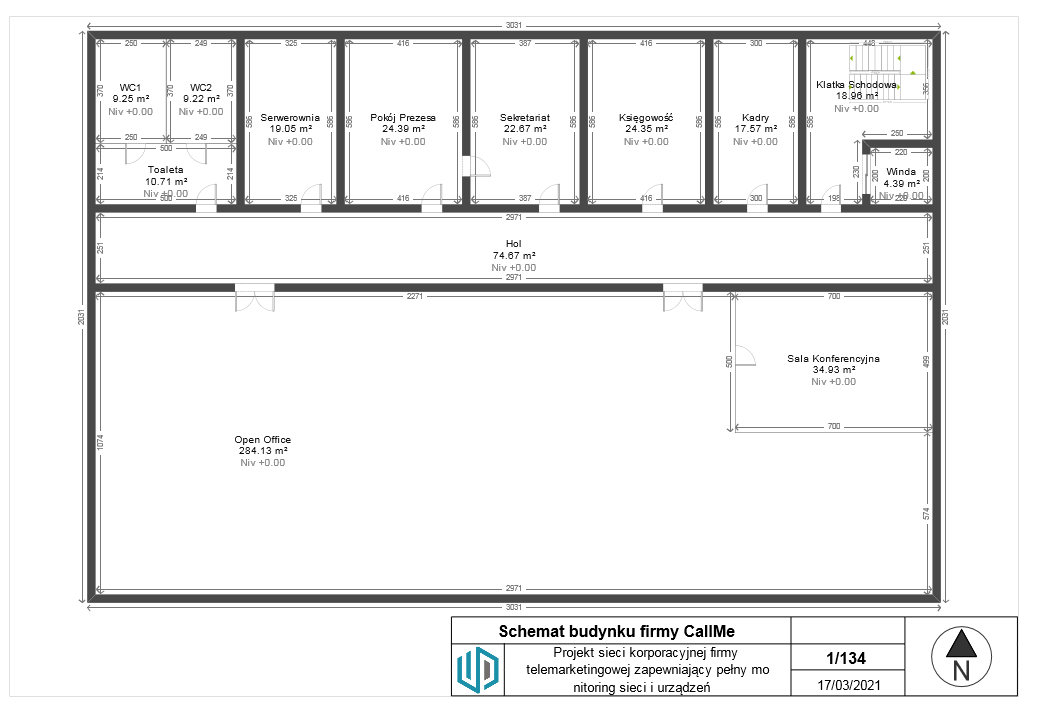
\includegraphics[width=.9\linewidth]{./data/siec/plan_budynku.png}
\end{center}
\end{frame}
\begin{frame}[label={sec:org0ae8d1f}]{Plan fizyczny sieci}
\begin{center}
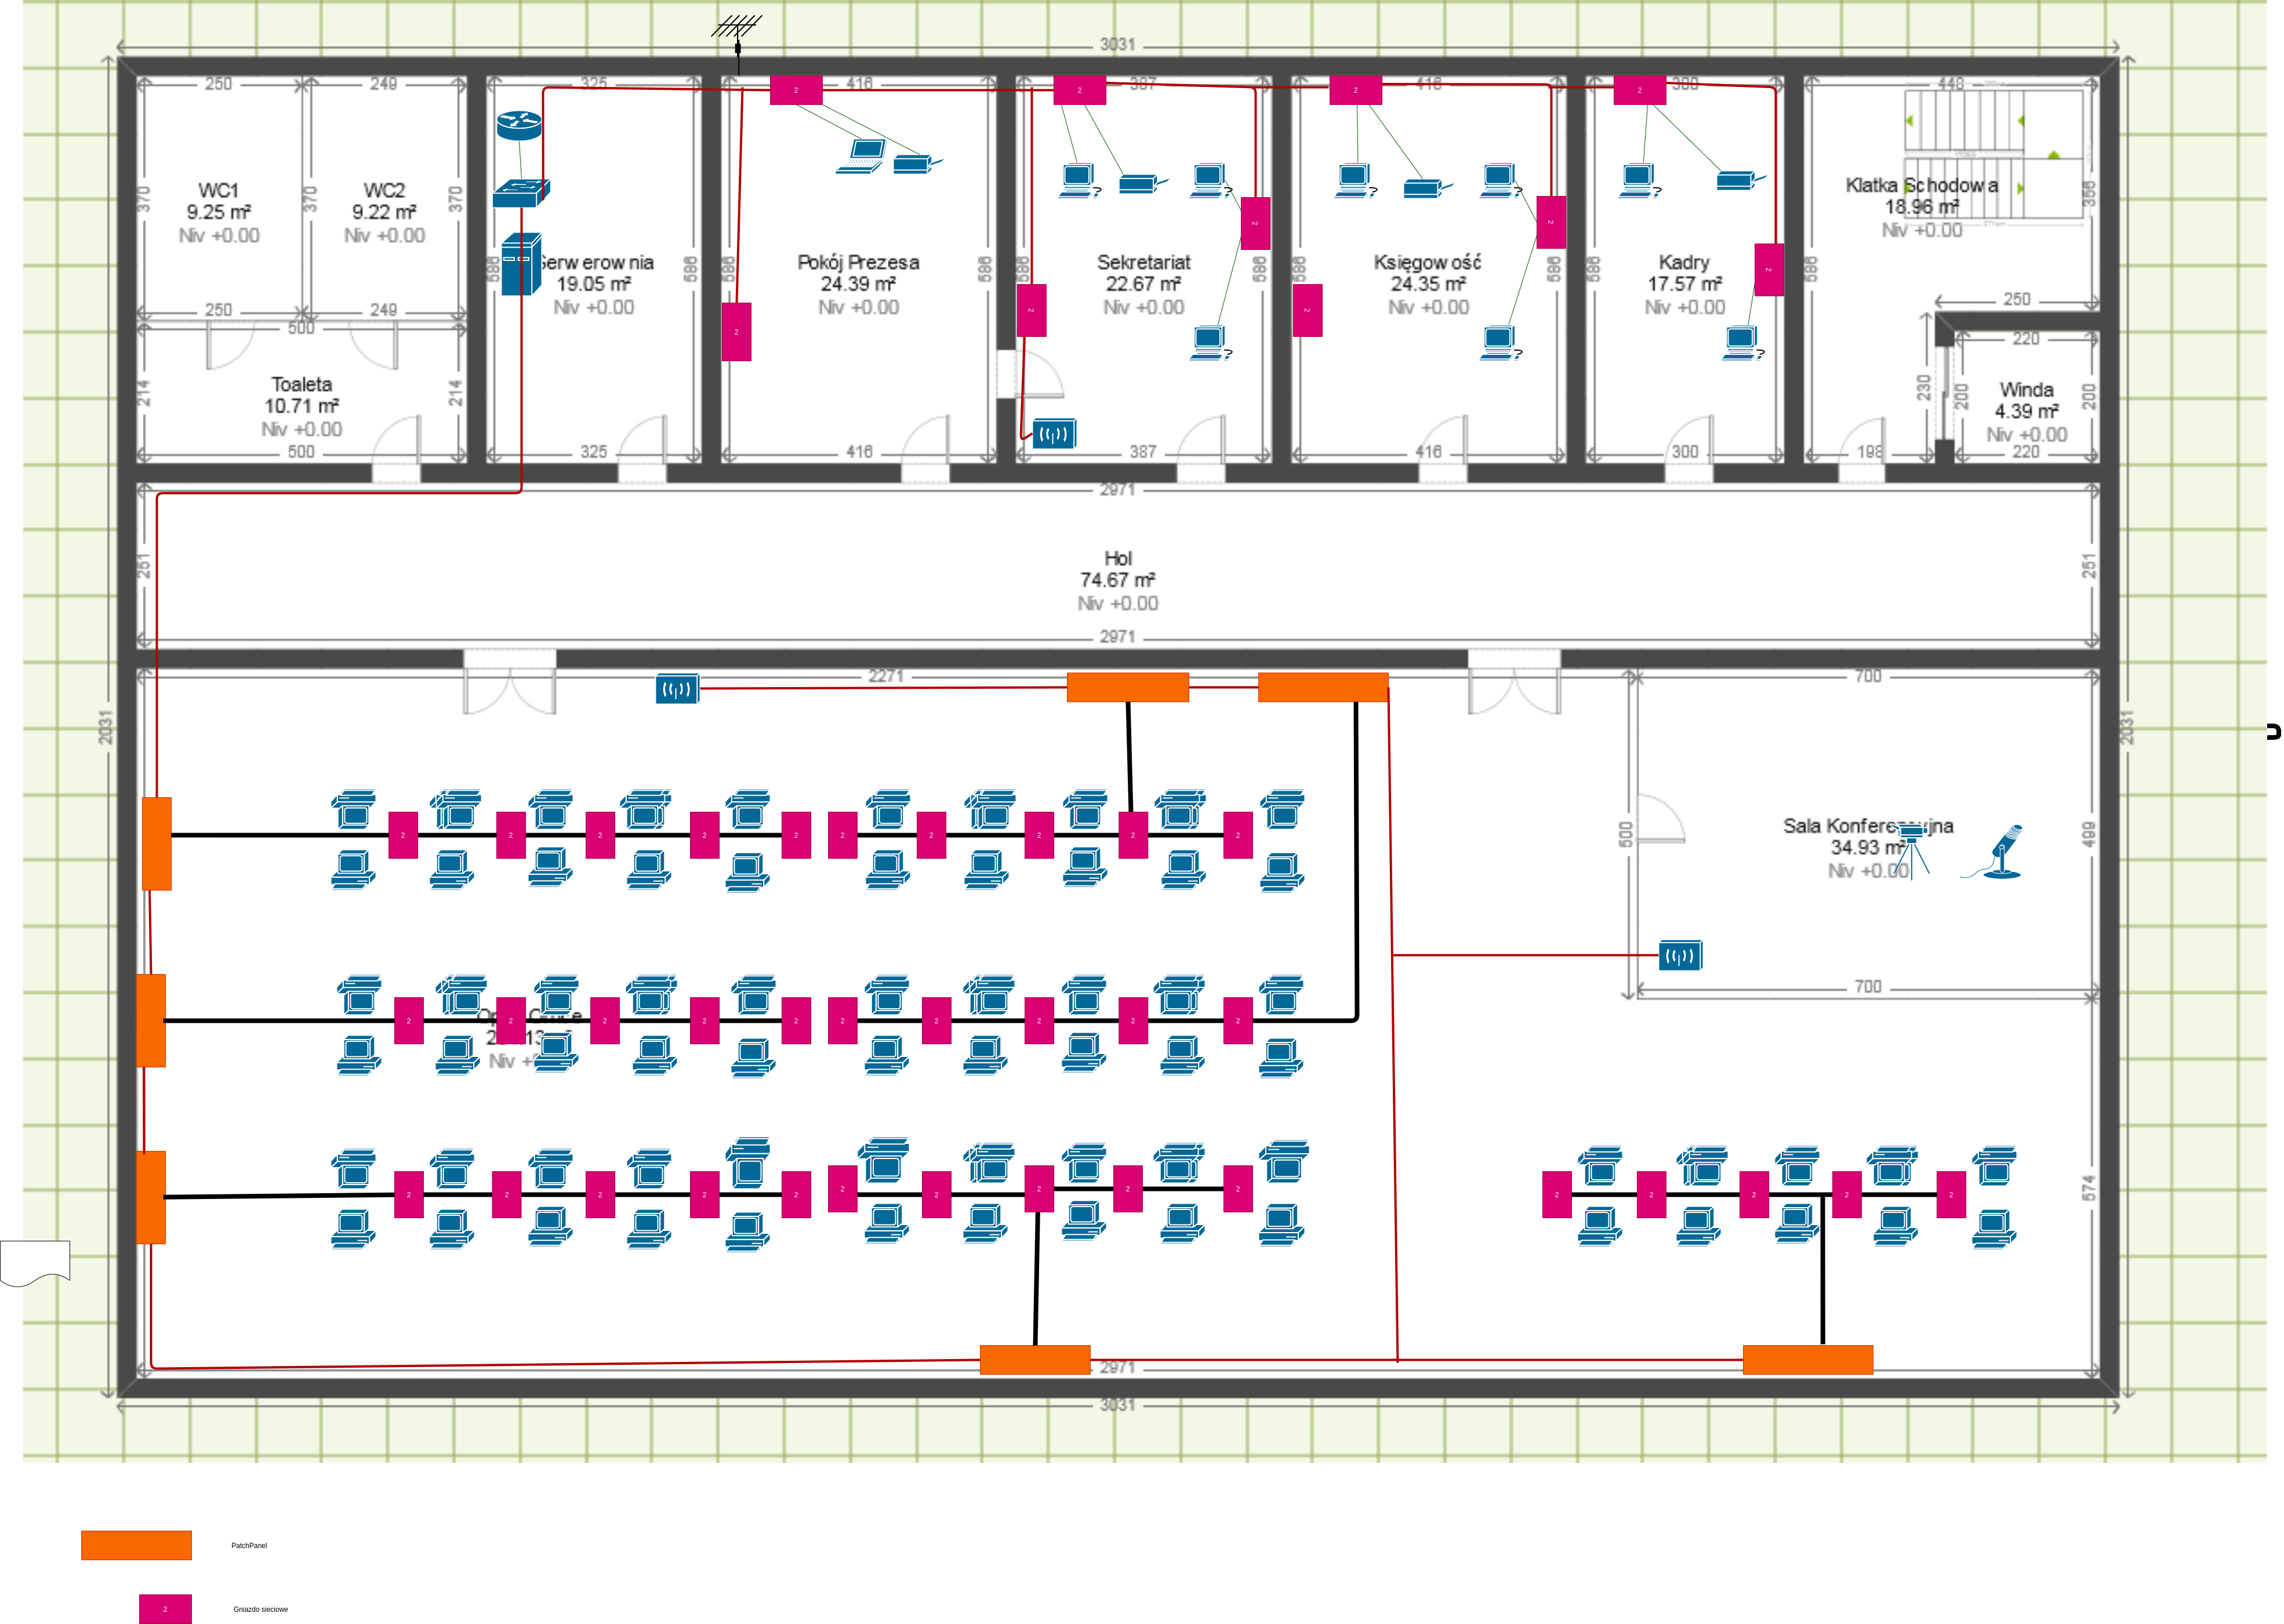
\includegraphics[width=.9\linewidth]{./data/siec/plan_fizyczny.png}
\end{center}
\end{frame}
\begin{frame}[label={sec:org759e2e1}]{Model Propagacyjny}
\begin{center}
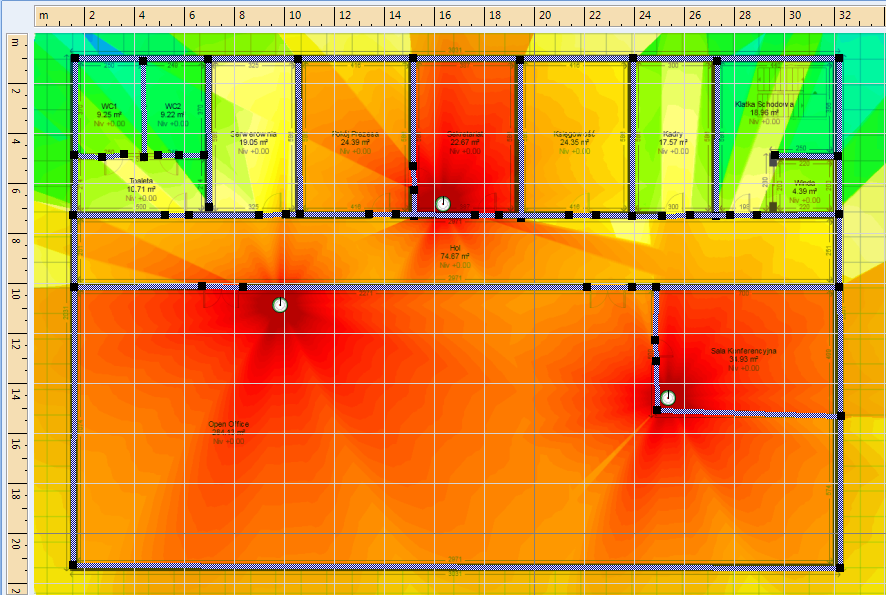
\includegraphics[width=.9\linewidth]{./data/siec/wifi.png}
\end{center}
\end{frame}
\begin{frame}[label={sec:orgb7354cf}]{Plan logiczny sieci}
\begin{center}
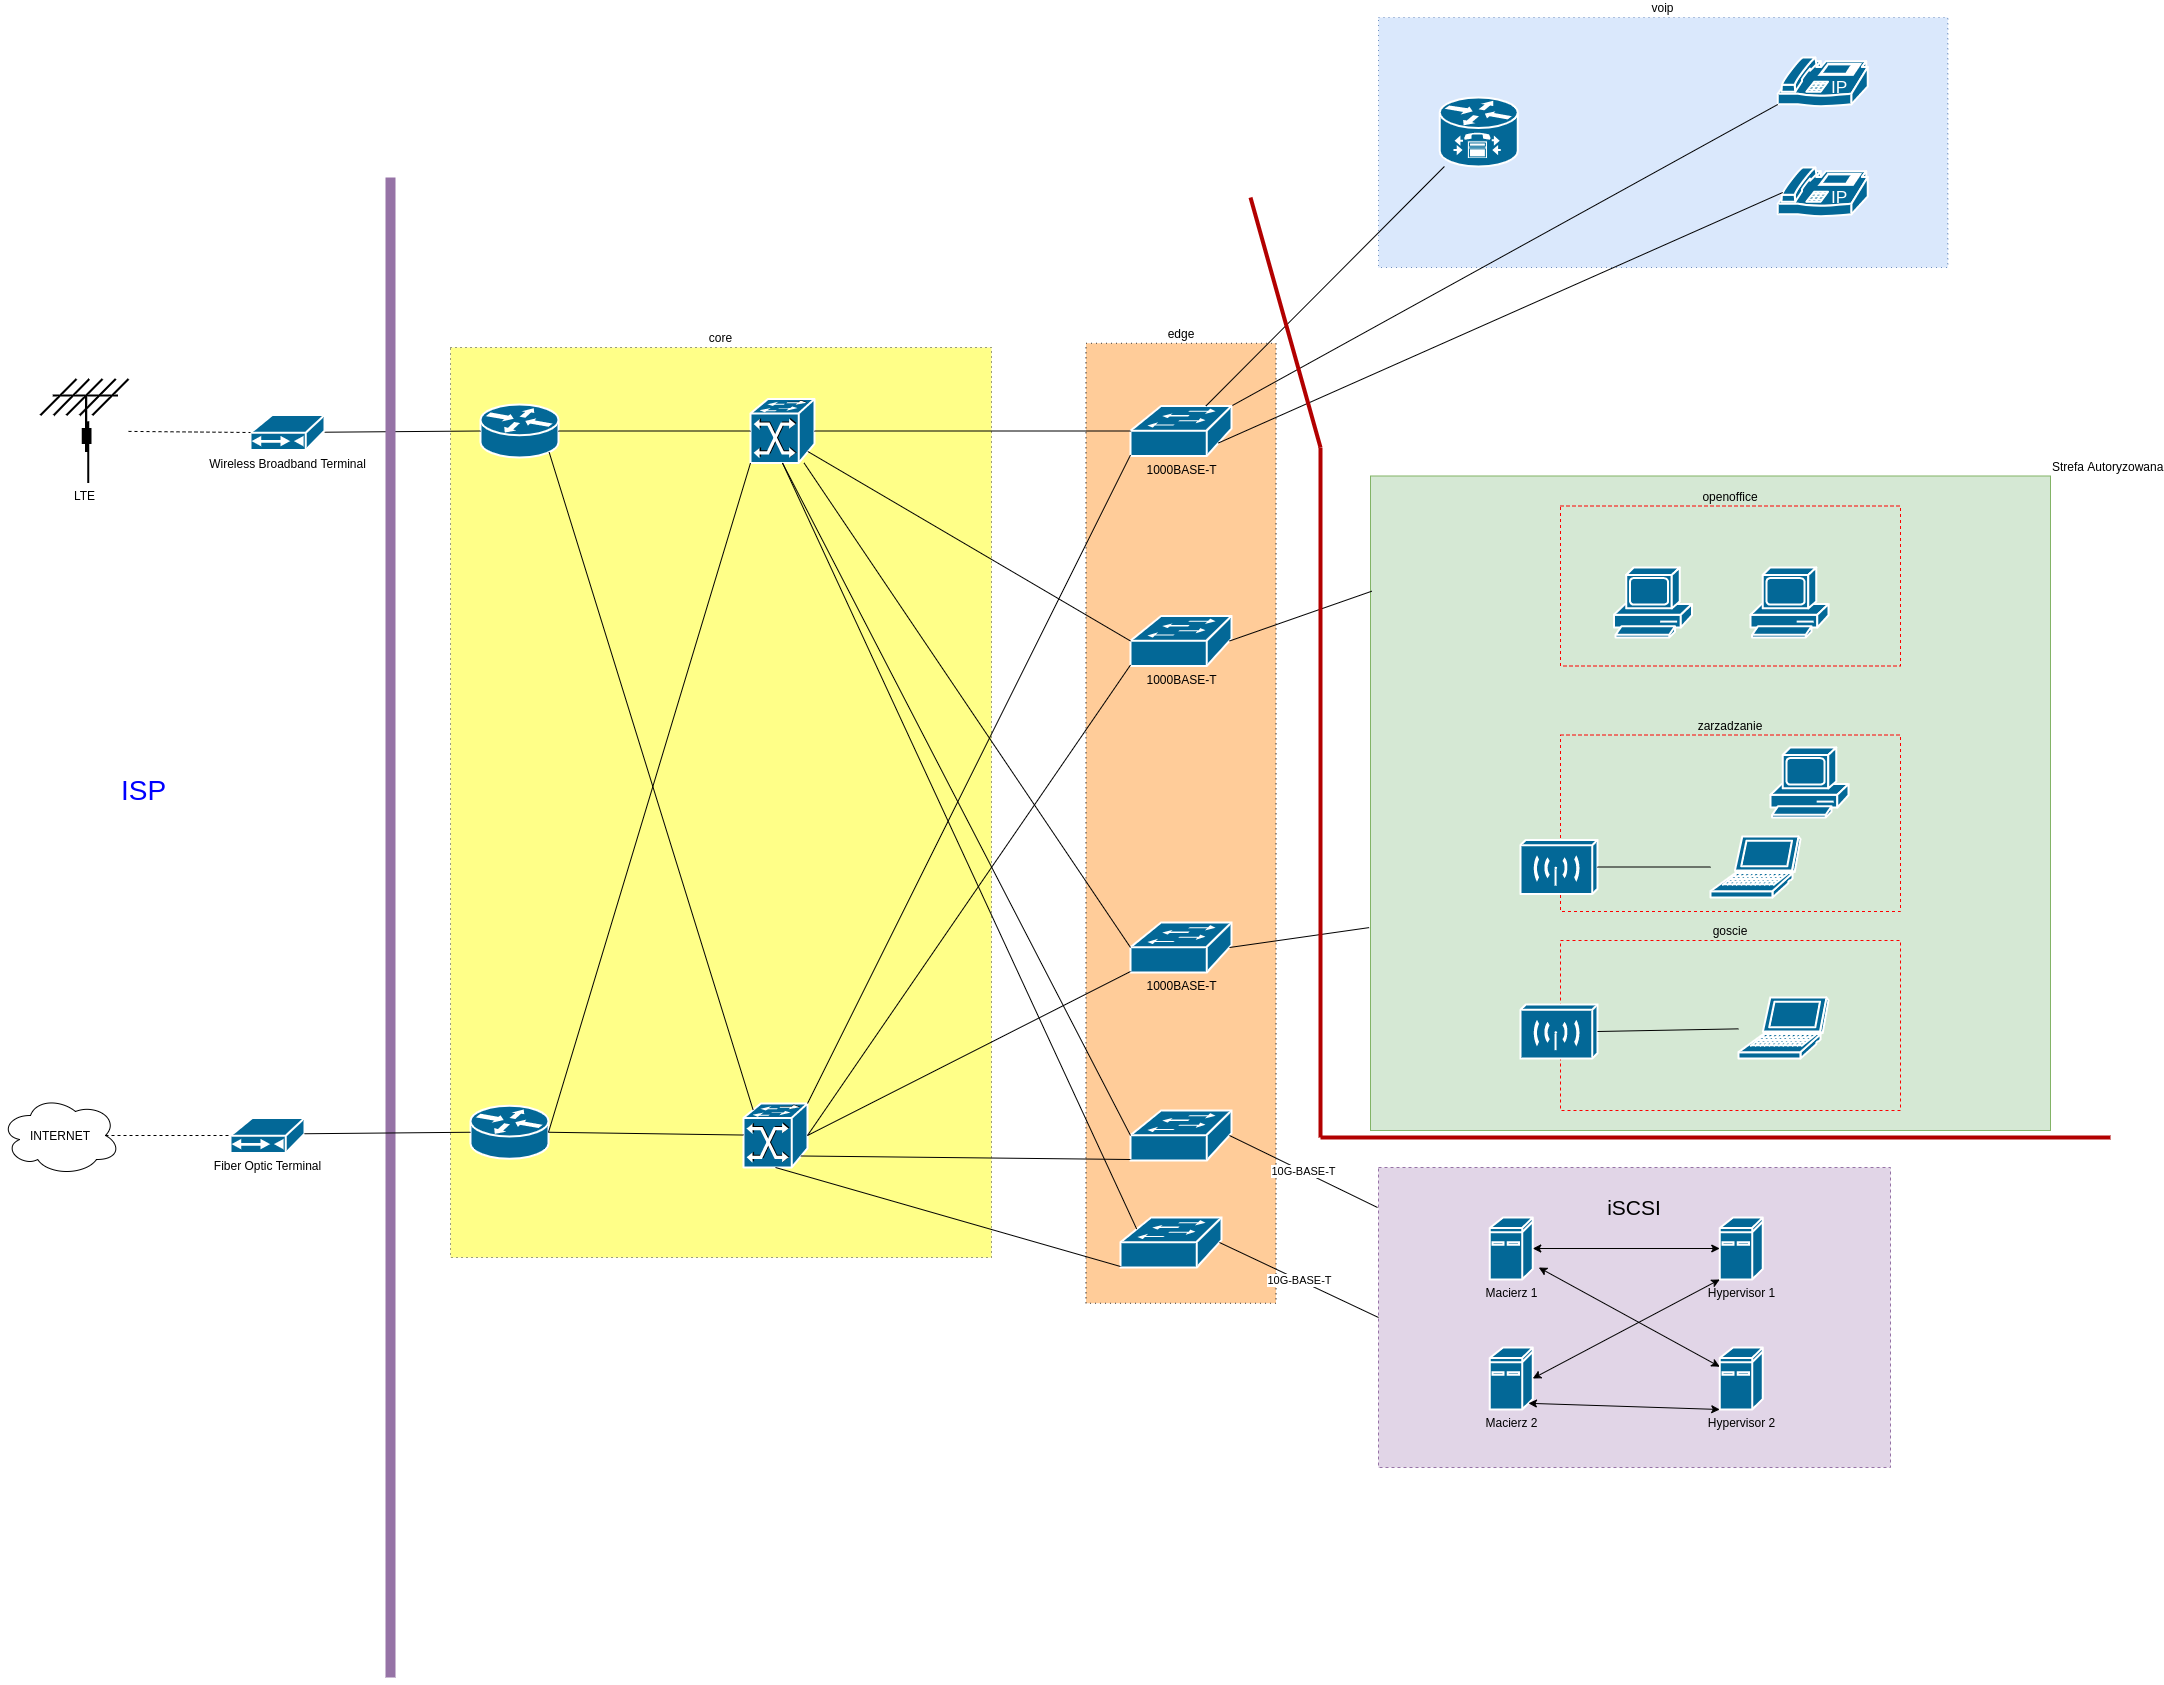
\includegraphics[width=.9\linewidth]{./data/siec/network_diagram_clean.png}
\end{center}
\end{frame}
\begin{frame}[label={sec:orga292552}]{Architektura serwerowa}
\begin{center}
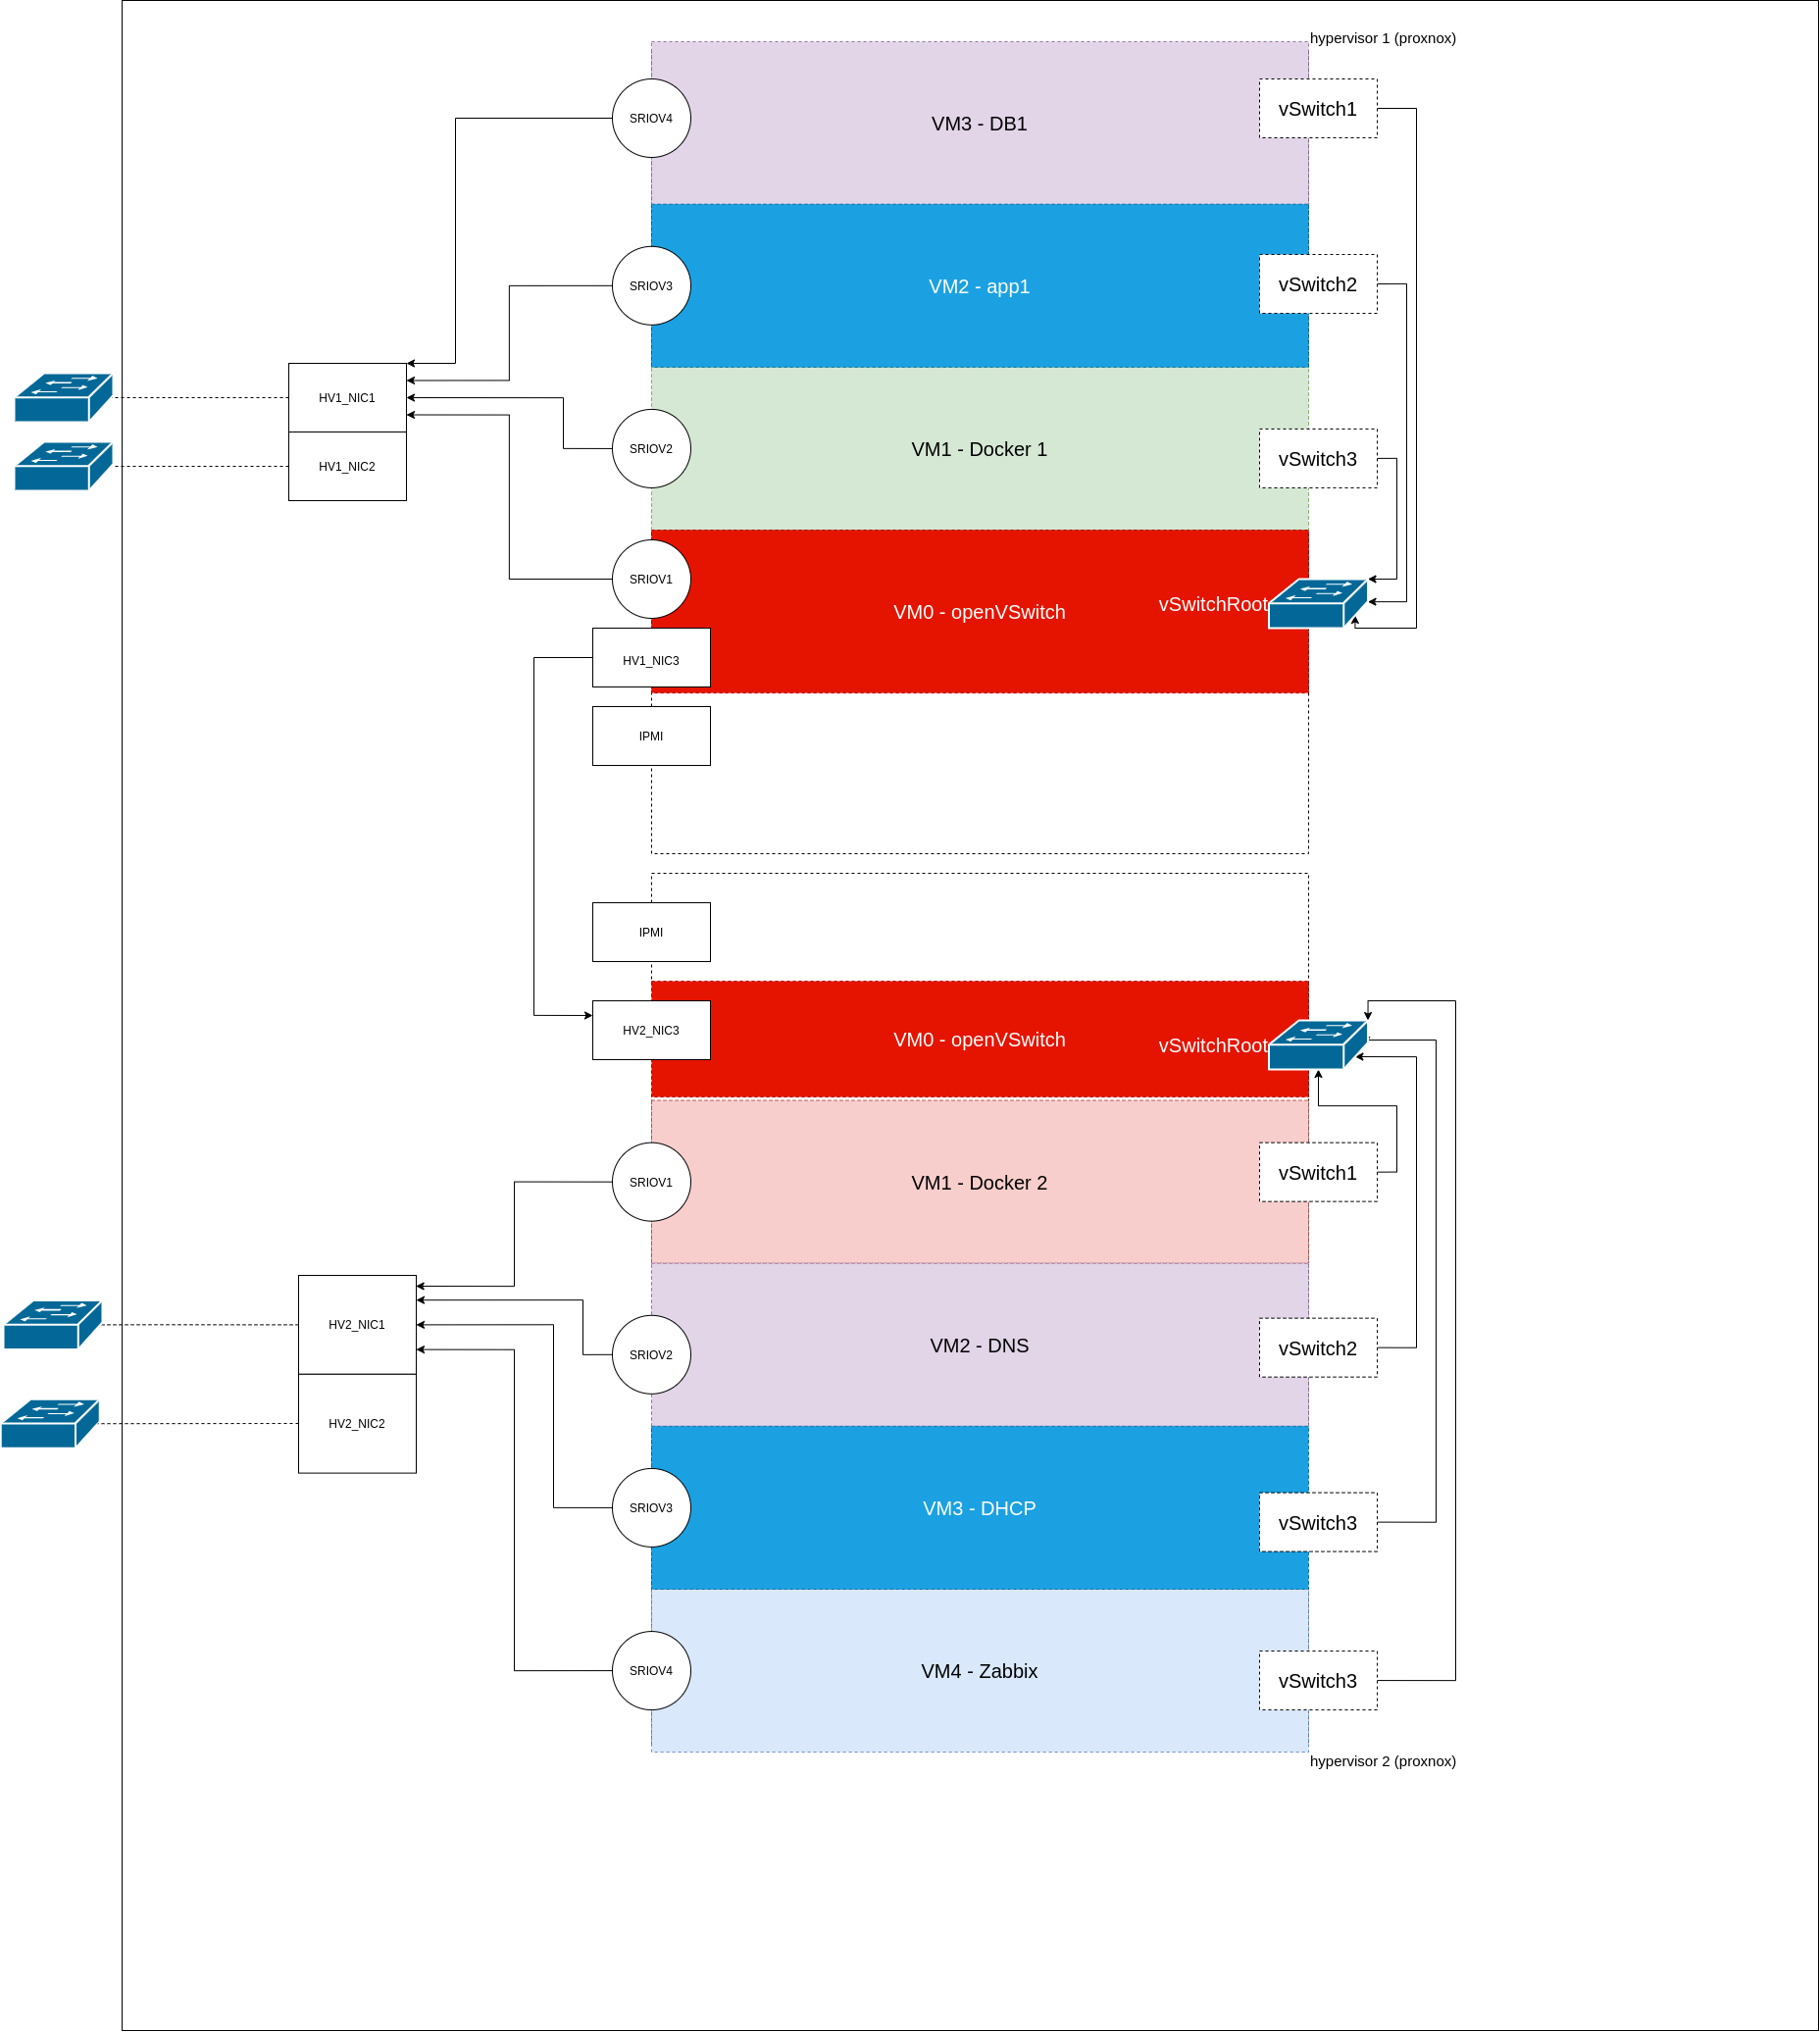
\includegraphics[width=.9\linewidth]{./data/siec/server_diagram.png}
\end{center}
\end{frame}
\section{App1/2}
\label{sec:orgddbd9c0}
\begin{frame}[label={sec:orgb6b4fac},fragile]{App1}
 \TINY
\begin{minted}[]{php}
<?php
$host = '192.168.200.132';
$db   = 'lab3'; $user = 'admin'; $pass = 'pwsz';
$port = '3306'; $charset = 'utf8';
$options = [
    \PDO::ATTR_ERRMODE            => \PDO::ERRMODE_EXCEPTION,
    \PDO::ATTR_DEFAULT_FETCH_MODE => \PDO::FETCH_ASSOC,
    \PDO::ATTR_EMULATE_PREPARES   => false,
];
$dsn = "mysql:host=$host;dbname=$db;charset=$charset;port=$port";
try {
     $pdo = new \PDO($dsn, $user, $pass, $options);
} catch (\PDOException $e) {
     throw new \PDOException($e->getMessage(), (int)$e->getCode());
}
$stmt = $pdo->query("SELECT * FROM aktorzy");
while ($row = $stmt->fetch()) {
    echo $row['nazwisko']."<br />\n";
}
?>
\end{minted}
\end{frame}
\begin{frame}[label={sec:org87114bc}]{App1 + db1}
\begin{columns}
\begin{column}{0.5\columnwidth}
\begin{block}{App1}
\begin{center}
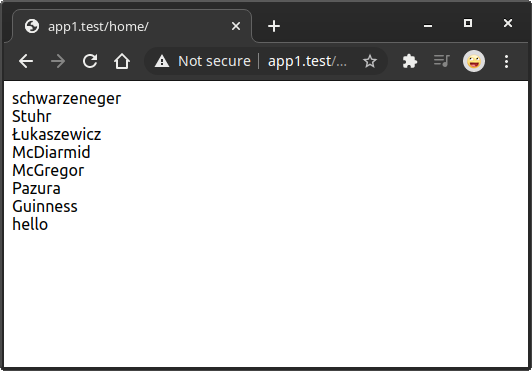
\includegraphics[width=.9\linewidth]{./data/app/app1.png}
\end{center}
\end{block}
\end{column}
\begin{column}{0.5\columnwidth}
\begin{block}{App1}
\begin{center}
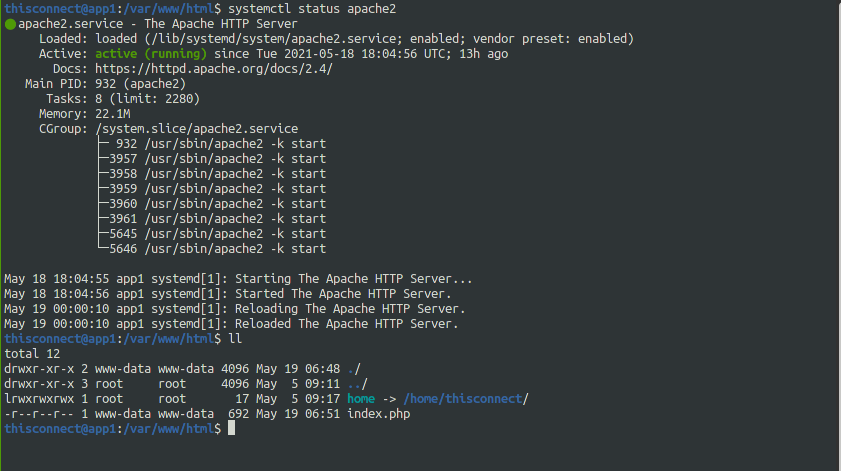
\includegraphics[width=.9\linewidth]{./data/app/app1status.png}
\end{center}
\end{block}
\end{column}
\end{columns}
\end{frame}
\begin{frame}[label={sec:org1e01d7b},fragile]{App2}
 \TINY
\begin{minted}[]{php}
<?php
$host = '192.168.200.145';
$db   = 'lab3'; $user = 'admin'; $pass = 'pwsz';
$port = '3306'; $charset = 'utf8';
$options = [
    \PDO::ATTR_ERRMODE            => \PDO::ERRMODE_EXCEPTION,
    \PDO::ATTR_DEFAULT_FETCH_MODE => \PDO::FETCH_ASSOC,
    \PDO::ATTR_EMULATE_PREPARES   => false,
];
$dsn = "mysql:host=$host;dbname=$db;charset=$charset;port=$port";
try {
     $pdo = new \PDO($dsn, $user, $pass, $options);
} catch (\PDOException $e) {
     throw new \PDOException($e->getMessage(), (int)$e->getCode());
}
$stmt = $pdo->query("SELECT * FROM filmy");
while ($row = $stmt->fetch()) {
    echo $row['tytul']." ".$row['rok']."<br />\n";
}
?>
\end{minted}
\end{frame}
\begin{frame}[label={sec:org32355de}]{App2 + db2}
\begin{center}
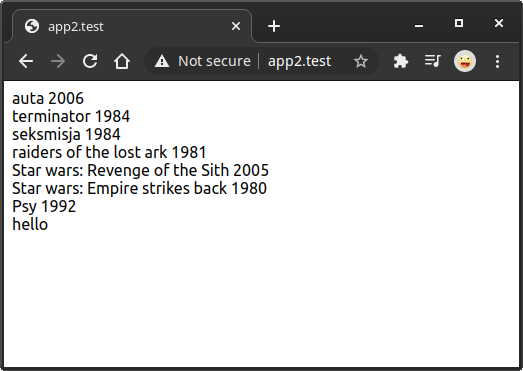
\includegraphics[width=.9\linewidth]{./data/app/app2.png}
\end{center}
\end{frame}
\section{Monitoring sieci}
\label{sec:orgbc1e0cc}
\begin{frame}[label={sec:org6b55831}]{Zabbix}
Zabbix jest rozwiązanie open-source (GPLv2) do monitorowania dużej ilości komponentów sieci komputerowej w tym:
\begin{itemize}
\item sieci
\item urządzeń sieciowych
\item stacji roboczych
\item serwerów
\item usług
\end{itemize}
\end{frame}
\begin{frame}[label={sec:orge51c02e}]{Zabbix}
\begin{center}
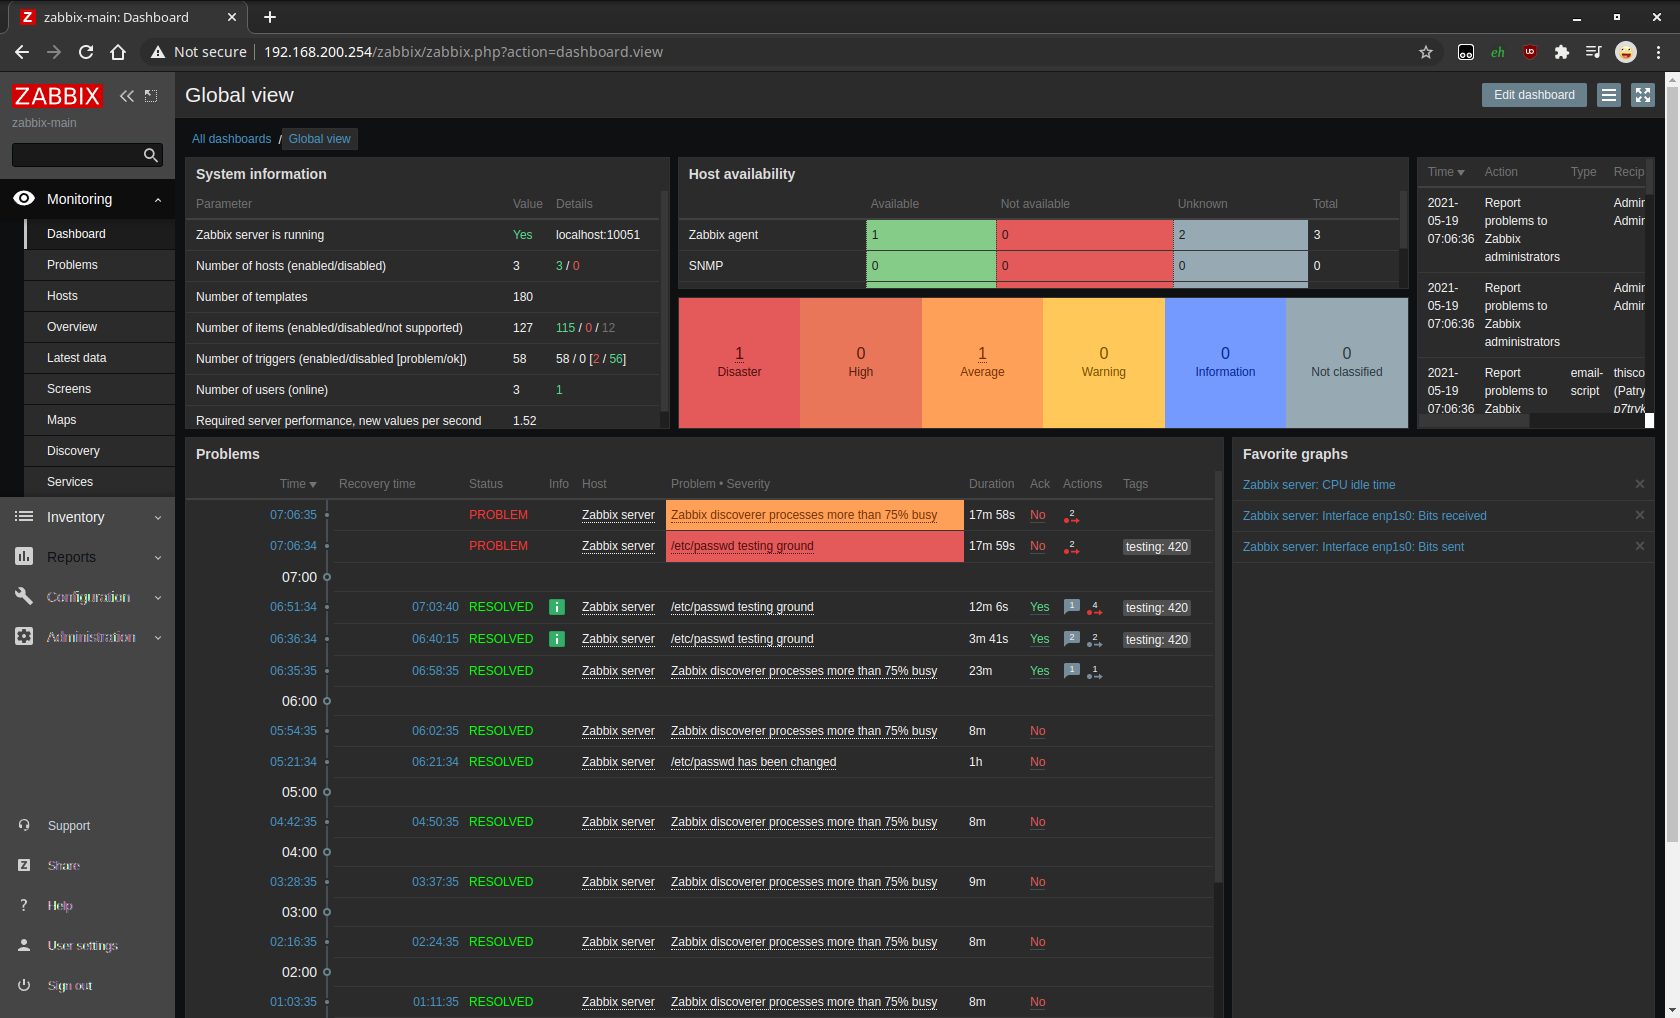
\includegraphics[width=.9\linewidth]{./data/zabbix/homepage.png}
\end{center}
\end{frame}
\begin{frame}[label={sec:orgc29a225}]{Triggery}
\begin{center}
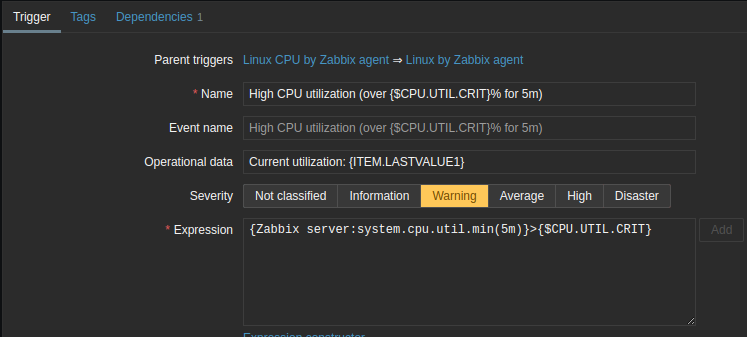
\includegraphics[width=.9\linewidth]{./data/zabbix/trigger2.png}
\end{center}
\end{frame}
\begin{frame}[label={sec:org5af56ad},fragile]{Powiadomienia}
 \begin{minted}[]{bash}
#!/bin/bash
# uzywajac ssmtp via mailserver
echo "sending mail" > /var/log/zabbix/custom.log
echo "$3" | /usr/bin/mail -s "$2" $1

exit 0
\end{minted}
\end{frame}
\begin{frame}[label={sec:org2ededa5}]{Powiadomienia (kont.)}
\begin{columns}
\begin{column}{0.55\columnwidth}
\begin{block}{Media type}
\begin{center}
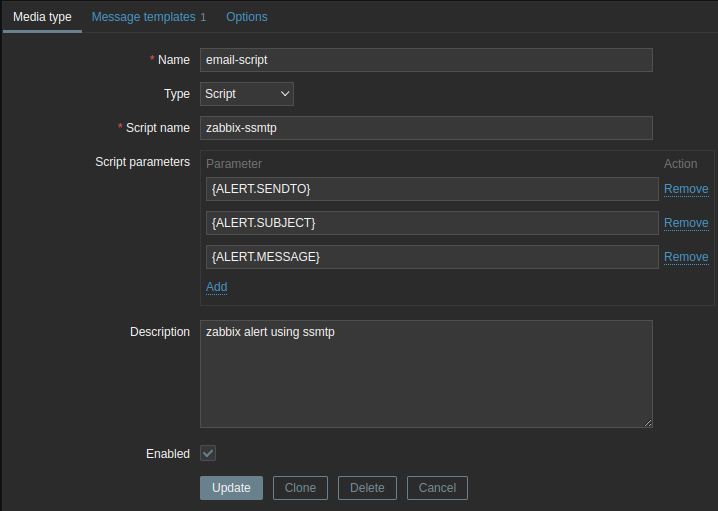
\includegraphics[width=.9\linewidth]{./data/zabbix/trigger.png}
\end{center}
\end{block}
\end{column}

\begin{column}{0.55\columnwidth}
\begin{block}{Efekt}
\begin{center}
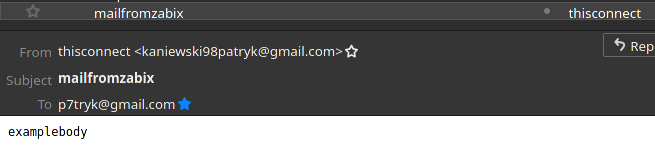
\includegraphics[width=.9\linewidth]{./data/zabbix/mail.png}
\end{center}
\end{block}
\end{column}
\end{columns}
\end{frame}

\begin{frame}[label={sec:orgc3e5286},fragile]{Powiadomienia (kont.)}
 \begin{columns}
\begin{column}{0.6\columnwidth}
\begin{block}{notify-send}
\begin{minted}[]{bash}
#!/bin/bash

ssh 192.168.200.1 "notify-send $1"
\end{minted}
\end{block}
\end{column}

\begin{column}{0.4\columnwidth}
\begin{block}{Efekt}
\begin{center}
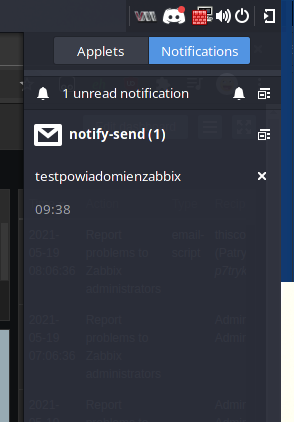
\includegraphics[width=.9\linewidth]{./data/zabbix/notify-send.png}
\end{center}
\end{block}
\end{column}
\end{columns}
\end{frame}
\section{Autoryzacja na poziomie sieci}
\label{sec:org46ca18f}
\begin{frame}[label={sec:org7b26984}]{802.1x}
\end{frame}
\section{DHCP}
\label{sec:orgeec1318}
\begin{frame}[label={sec:org5c39ba0}]{DHCP}
\begin{columns}
\begin{column}{0.55\columnwidth}
\begin{block}{Master}
\begin{center}
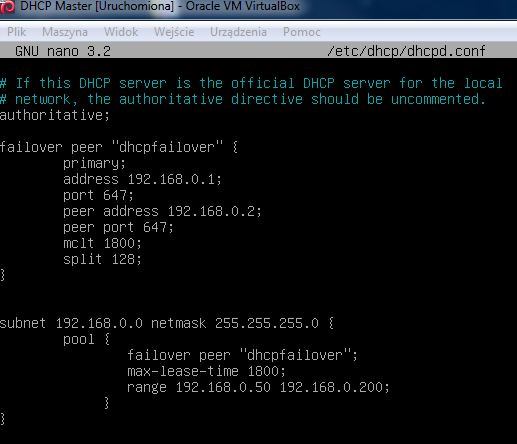
\includegraphics[width=.9\linewidth]{./data/dhcp/5_master.png}
\end{center}
\end{block}
\end{column}
\begin{column}{0.55\columnwidth}
\begin{block}{Slave}
\begin{center}
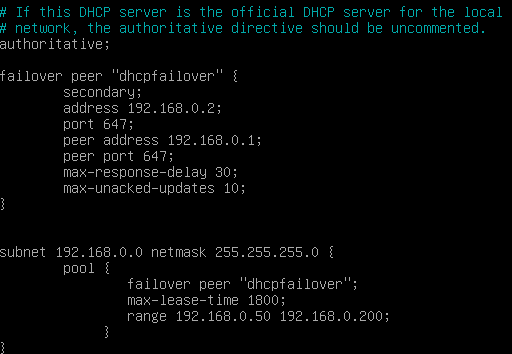
\includegraphics[width=.9\linewidth]{./data/dhcp/5_slave.png}
\end{center}
\end{block}
\end{column}
\end{columns}

\begin{block}{lease}
\begin{center}
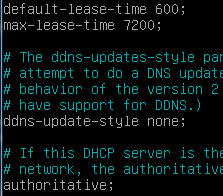
\includegraphics[width=.9\linewidth]{./data/dhcp/5_small.png}
\end{center}
\end{block}
\end{frame}
\begin{frame}[label={sec:org0deb090}]{Failover}
Do poprawnego działania usługi DHCP Failover wymagane jest aby obydwa serwery miały ustawione takie same daty oraz czas:
\begin{center}

\includegraphics[width=.9\linewidth]{./data/dhcp/6_czas.png}
\end{center}
\end{frame}
\begin{frame}[label={sec:orgec0b08a}]{}
\begin{columns}
\begin{column}{0.55\columnwidth}
\begin{block}{Slave}
\begin{center}
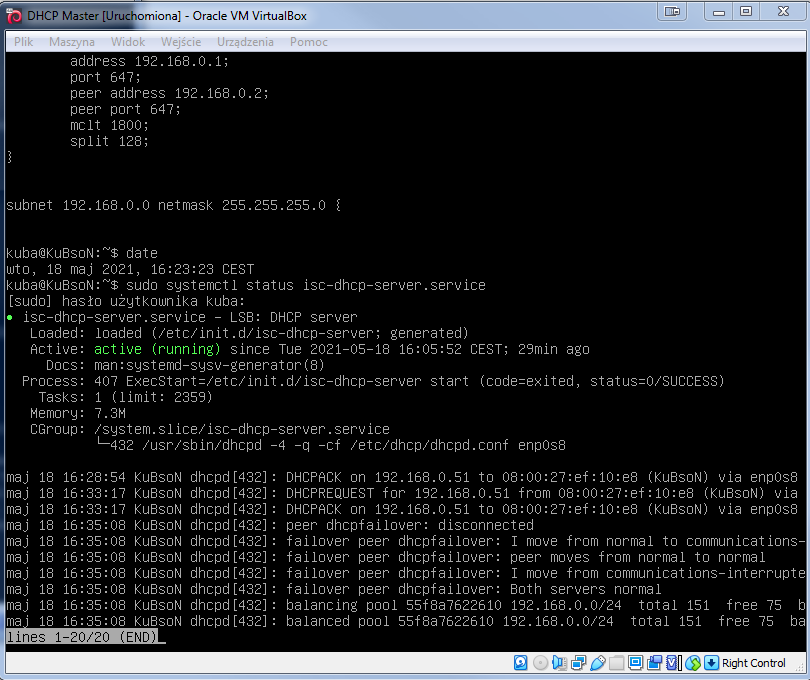
\includegraphics[width=.9\linewidth]{./data/dhcp/7_master.png}
\end{center}
\end{block}
\end{column}
\begin{column}{0.55\columnwidth}
\begin{block}{Master}
\begin{center}
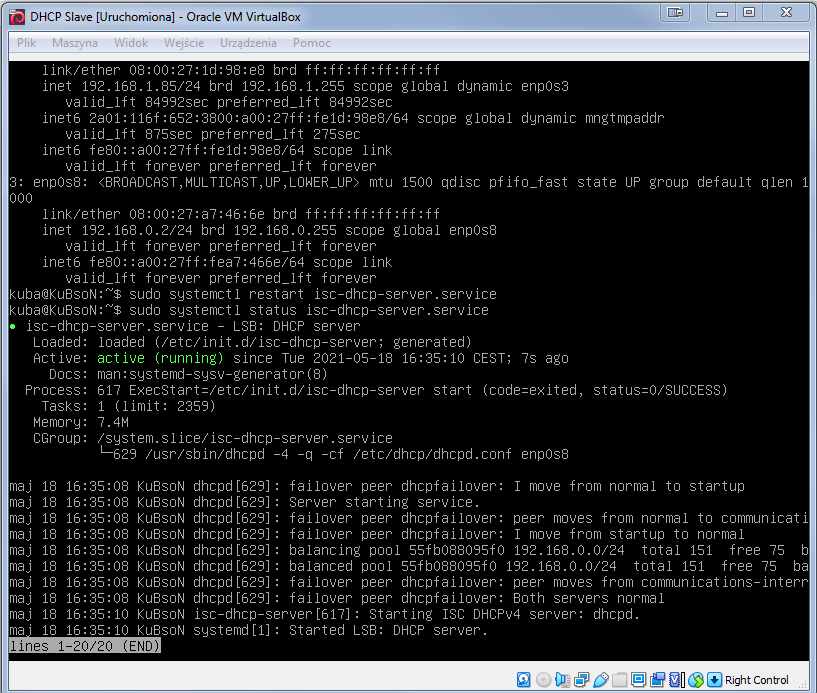
\includegraphics[width=.9\linewidth]{./data/dhcp/7_slave.png}
\end{center}
\end{block}
\end{column}
\end{columns}
\end{frame}
\begin{frame}[label={sec:org4423da7}]{klient}
\begin{columns}
\begin{column}{0.55\columnwidth}
\begin{block}{interface}
\begin{center}
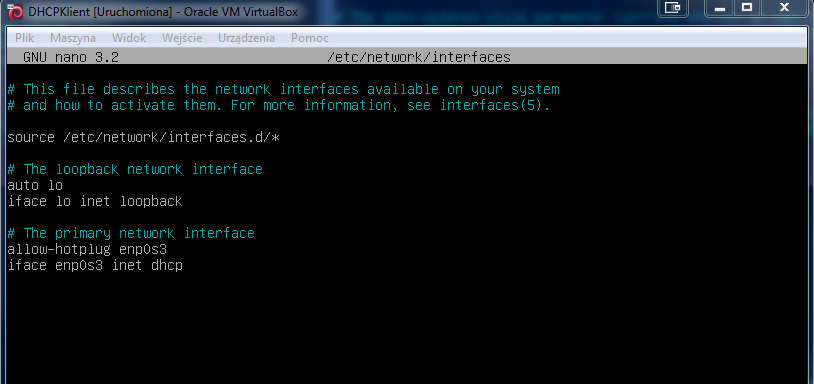
\includegraphics[width=.9\linewidth]{./data/dhcp/8_1.png}
\end{center}
\end{block}
\end{column}
\begin{column}{0.55\columnwidth}
\begin{block}{ip a}
\begin{center}
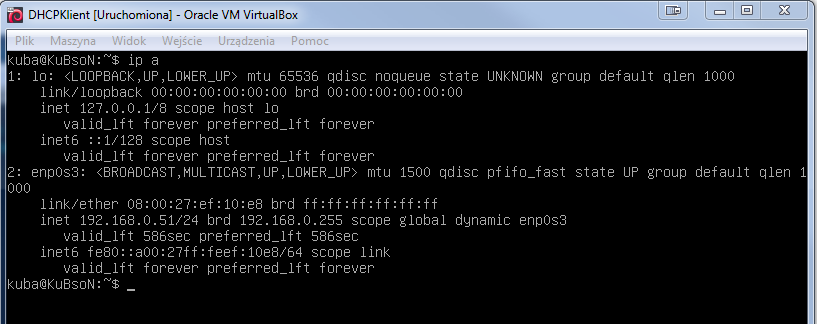
\includegraphics[width=.9\linewidth]{./data/dhcp/8_2.png}
\end{center}
\end{block}
\end{column}
\end{columns}
\end{frame}
\begin{frame}[label={sec:orgddeabf9}]{DHCP leases}
Jak można zobaczyć dane zostaly zsynchronizowane na obydwu serwerach
\begin{columns}
\begin{column}{0.55\columnwidth}
\begin{block}{Master}
\begin{center}
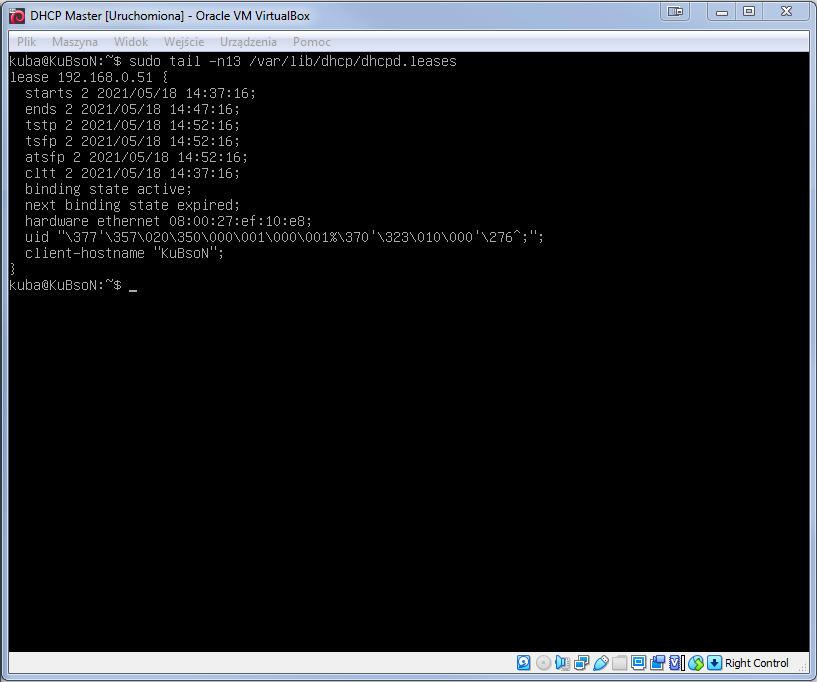
\includegraphics[width=.9\linewidth]{./data/dhcp/9_master.png}
\end{center}
\end{block}
\end{column}
\begin{column}{0.55\columnwidth}
\begin{block}{Slave}
\begin{center}
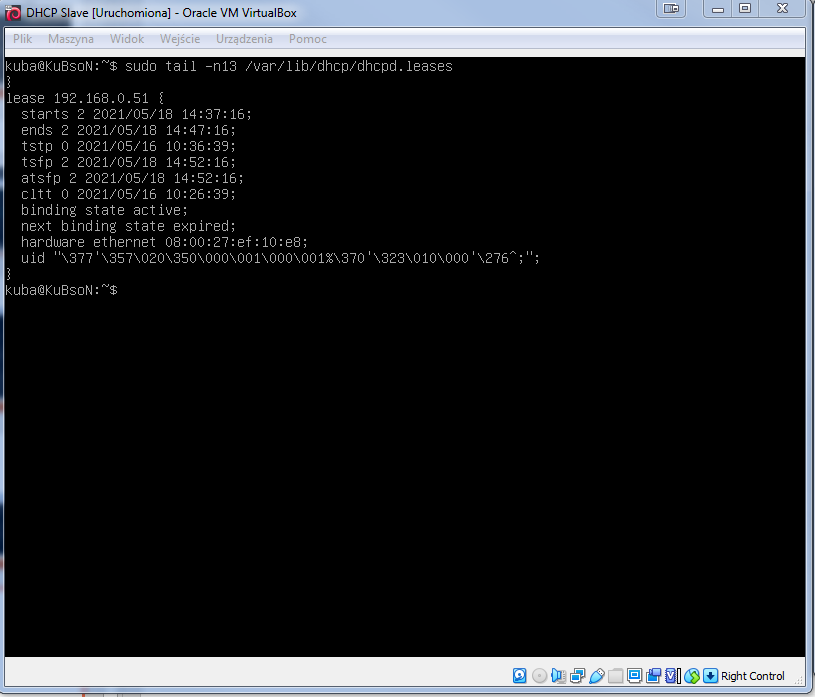
\includegraphics[width=.9\linewidth]{./data/dhcp/9_slave.png}
\end{center}
\end{block}
\end{column}
\end{columns}
\end{frame}
\begin{frame}[label={sec:orga3a1c21}]{}
\begin{center}
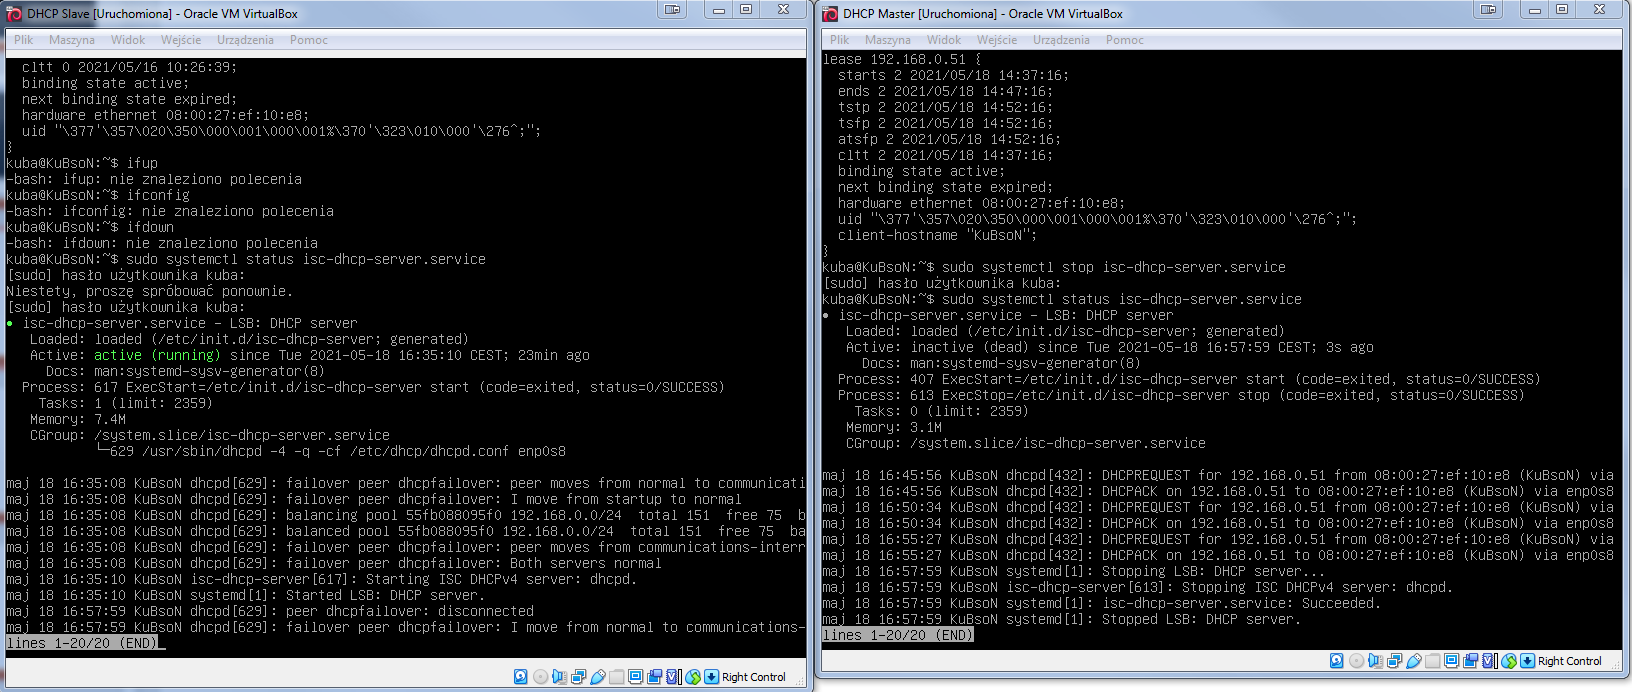
\includegraphics[width=.9\linewidth]{./data/dhcp/10_slave.png}
\end{center}
\end{frame}
\begin{frame}[label={sec:orgb1c5858}]{}
\begin{columns}
\begin{column}{0.55\columnwidth}
\begin{block}{Master}
\begin{center}
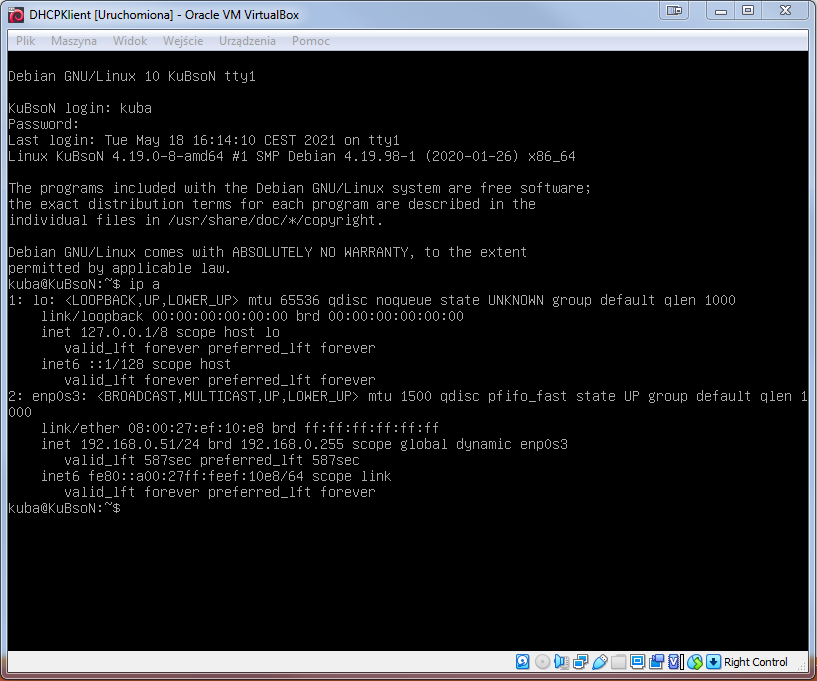
\includegraphics[width=.9\linewidth]{./data/dhcp/11_master.png}
\end{center}
\end{block}
\end{column}
\begin{column}{0.55\columnwidth}
\begin{block}{Slave}
\begin{center}
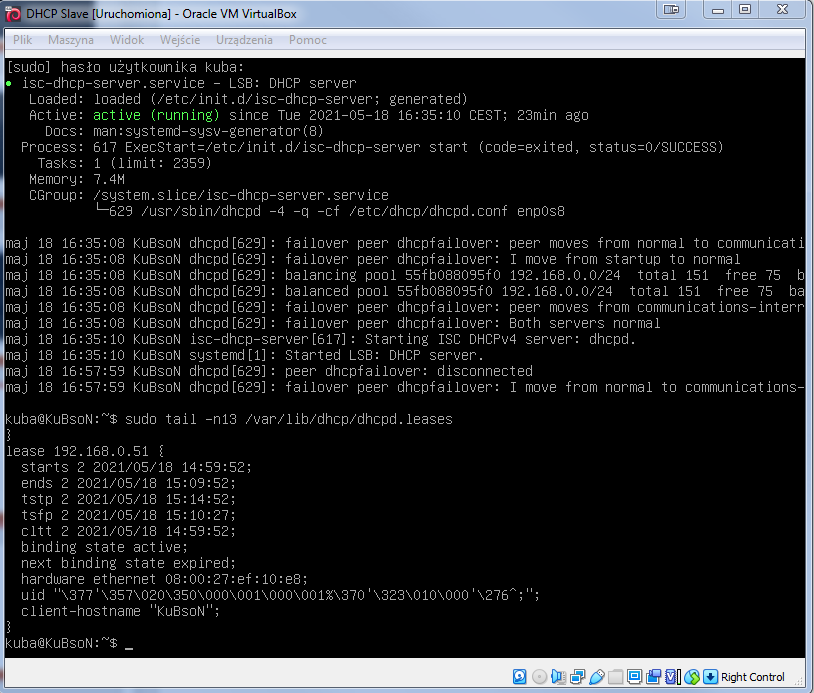
\includegraphics[width=.9\linewidth]{./data/dhcp/11_slave.png}
\end{center}
\end{block}
\end{column}
\end{columns}
\end{frame}
\section{DNS}
\label{sec:org94e1a56}
\begin{frame}[label={sec:org746ea97}]{Tworzenie Forward i Reverse Zone w pliku named.conf.local na Master}
\begin{center}
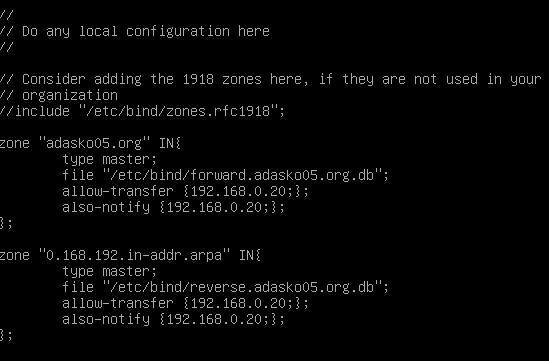
\includegraphics[width=.9\linewidth]{./data/dns/1.png}
\end{center}
\end{frame}
\begin{frame}[label={sec:org768a147}]{Tworzenie Forward Zone na Master}
\begin{center}
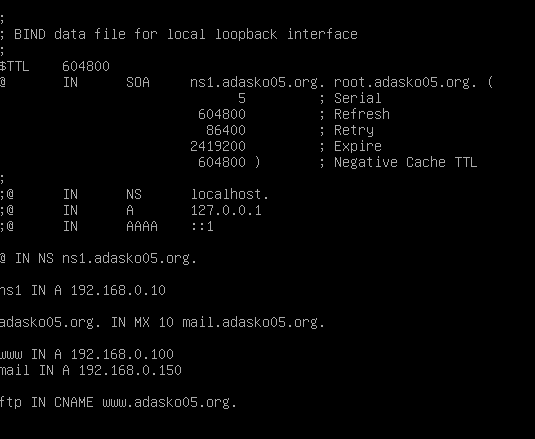
\includegraphics[width=.9\linewidth]{./data/dns/2.png}
\end{center}
\end{frame}
\begin{frame}[label={sec:org55d7923}]{Tworzenie Reverse Zone na Master}
\begin{center}
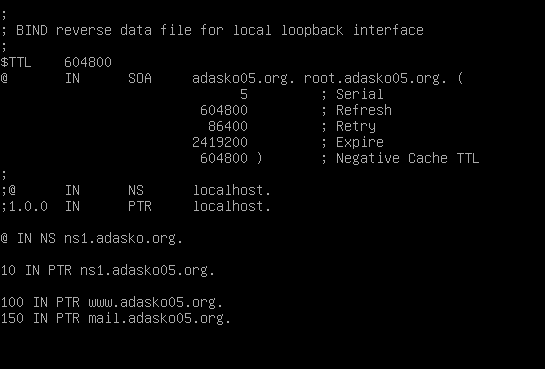
\includegraphics[width=.9\linewidth]{./data/dns/3.png}
\end{center}
\end{frame}
\begin{frame}[label={sec:org4d01ab4}]{Tworzenie Forward i Reverse Zone w pliku named.conf.local na Slave}
\begin{center}
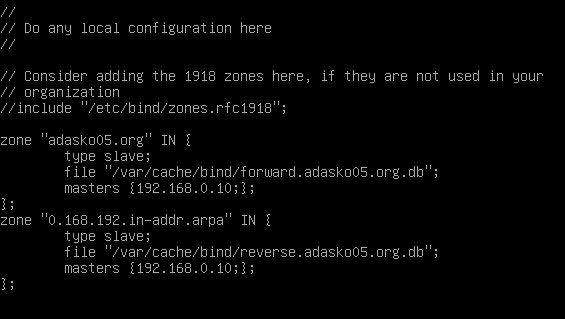
\includegraphics[width=.9\linewidth]{./data/dns/4.png}
\end{center}
\end{frame}
\begin{frame}[label={sec:org9c1ac8b}]{Status bind9 (DNS) Master}
\begin{center}
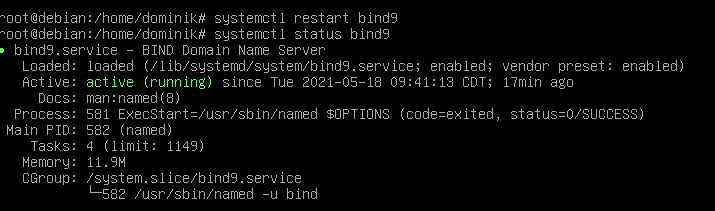
\includegraphics[width=.9\linewidth]{./data/dns/5.png}
\end{center}
\end{frame}
\begin{frame}[label={sec:orga729c4c}]{Status bind9 (DNS) Slave}
\begin{center}
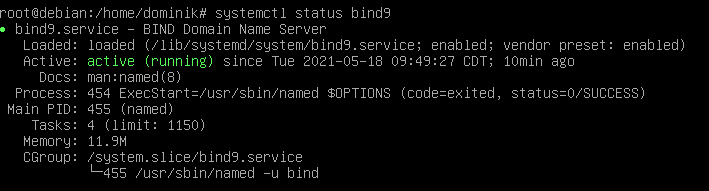
\includegraphics[width=.9\linewidth]{./data/dns/6.png}
\end{center}
\end{frame}
\section{Podsumowanie}
\label{sec:org3bc7190}
\begin{frame}[label={sec:org713f1b3}]{Podsumowanie}
\end{frame}
\end{document}
